% !TEX root = thesis.tex

% Front cover
% \includepdf{cover-front.pdf}

% Half-title
\maketitle


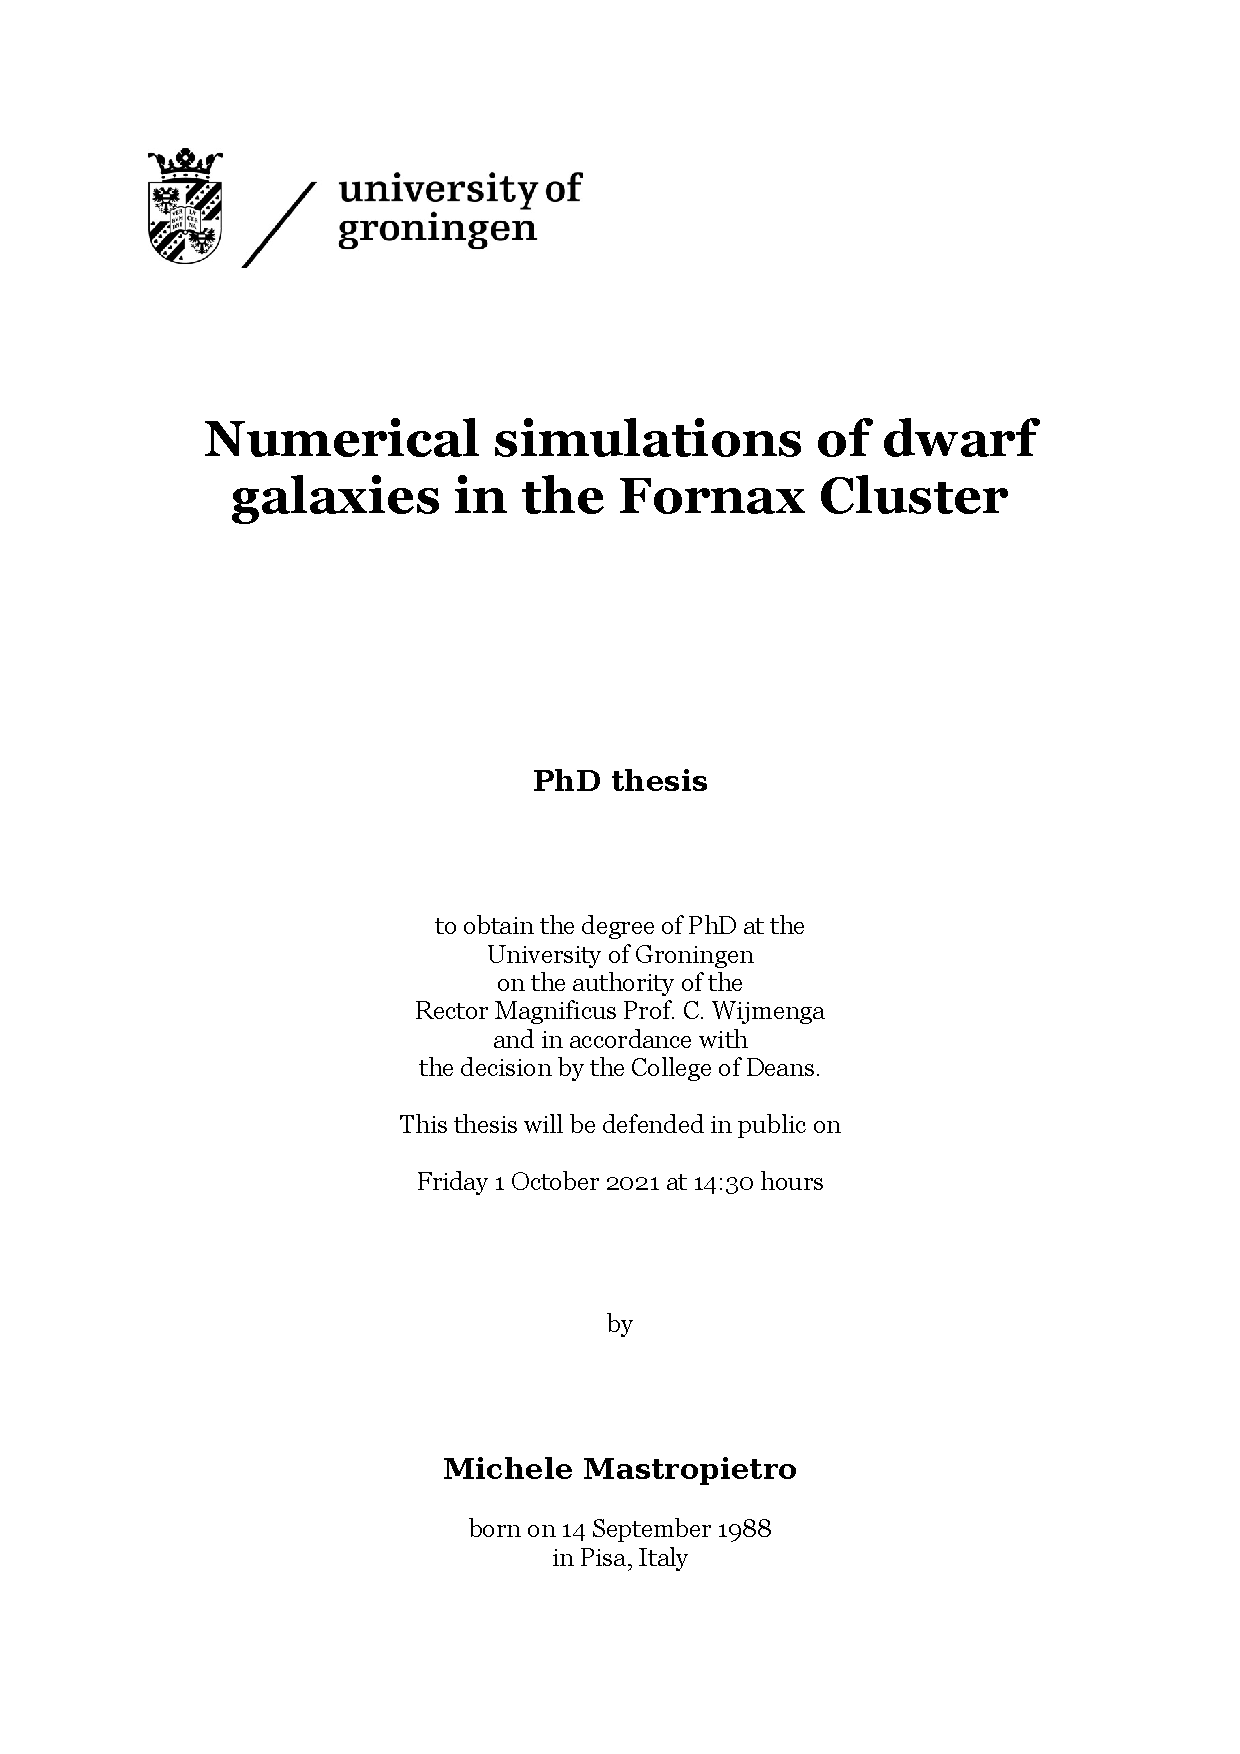
\includepdf[pages=-]{title_page.pdf}


\begin{comment}
% Official title
\begin{titlepage}
\null%
\label{thesis:title}
\vspace{3em}%
\pdfbookmark[1]{Title}{thesis:title}
\begin{center}

%% Skip space as in half-title
\vspace*{4\baselineskip}

%% Print the title.
\makeatletter
{\huge\@title}
\makeatother
\vfill

{\Large Proefschrift}

\medskip

{voorgedragen tot het behalen van \\
de graad van
Doctor in de Fysica en Sterrenkunde}


\medskip

door

\medskip

\makeatletter
{\Large \@author}
\makeatother

\medskip

aan de\\
{\large Universiteit Gent}\\
en aan de\\
{\large Rijksuniversiteit Groningen}\\
% Graduate School of Science and Engineering\\

\end{center}
\end{titlepage}





% Official verso
\clearpage
\thispagestyle{empty}
\null%
\label{thesis:committee}
\vfill
\pdfbookmark[1]{Doctoral committee}{thesis:committee}

% \noindent Members of the examination board:

\medskip\noindent
\begin{tabular}{@{}lll@{}}{Promotors:}\\\\
  \quad{}Prof.\ dr. Sven De Rijcke & Ghent University & (promotor)\\
  \quad{}Prof.\ dr. Michael\ Biehl & University of Groningen & (promotor)\\
  \quad{}Prof.\ dr. Reynier\ Peletier & University of Groningen & (promotor)\\
\\\\
\multicolumn{2}{@{}l@{}}{Composition of the Joint Evaluation Committee:} \\
\\
%   \quad{}Prof.\ dr.\  & chairperson \\
   \quad{}Prof.\ dr.\ Frazer Pearce & University of Nottingham\\
   \quad{}Prof.\ dr.\ Arjen van der Wel & Ghent University \\
   \quad{}Prof.\ dr.\ John McKean & University of Groningen \\
   \quad{}Prof.\ dr.\ Hugues Talbot & Université Paris-Saclay\\
\medskip\noindent
%   \quad{}Dr.\ & University of Groningen\\
% \\
% \multicolumn{2}{@{}l@{}}{Independent members:} \\
% \\
%   \quad{}Prof.\ dr.\ & University of Technology \\
%   \quad{}Prof.\ dr.\ & University \\
%   \quad{}Dr.\& University \\
% \\
% \multicolumn{2}{@{}l@{}}{Other member:} \\
% \\
%   \quad{}Dr.\ & ...\\
\end{tabular}
\end{comment}



% Copyright page
\clearpage
\thispagestyle{empty}
\null%
\label{thesis:colophon}
\vfill
\pdfbookmark[1]{Colophon}{thesis:colophon}
\noindent Written in 2021 by {\makeatletter{\@author}\makeatother}.\\
\textbf{Copyright}~\cczero{} The template for the layout of this thesis was inspired by my colleague Sam Verstocken who used the template of the dissertation of \href{ken.mx}{Ken Arroyo Ohori},
which was released into the public domain using the Creative~Commons~\cczero{}~code.
To view a copy of the \cczero{}~code, visit:\\\url{http://creativecommons.org/publicdomain/zero/1.0/}\\
\textbf{Colophon}
% This thesis was typeset with \XeTeX, Version 3.14159265-2.6-0.99998 (TeX Live 2017/Debian) using the \mbox{{\fanciestfont{}Feijoa}}, \texttt{GT Pressura} and $\mathrm{Asana\ Math}$ typefaces.
Most of the figures were created using \href{http://ipe.otfried.org/}{Ipe} (Copyright © 1993–2020 Otfried Cheong).
The source code of this thesis is available at: \\
\url{https://github.com/elehcim/phd-thesis}\\
\textbf{Cover}
...\\[2ex]
This research was funded by the European Union's Horizon 2020 research and innovation programme under the Marie Sk\l odowska-Curie
% Skłodowska-Curie
grant agreement N.~721463 to the \href{www.astro.rug.nl/~sundial}{SUNDIAL ITN network}.
\begin{figure*}[bh!]
  \centering
  
\includegraphics[width=0.2\textwidth]{EUflag}
\end{figure*}
